\documentclass{article}

\usepackage{mathtools,amsfonts}
\usepackage{enumerate}
\usepackage{fullpage}
\usepackage{array}
\usepackage{fancyvrb}

\begin{document}
\thispagestyle{empty}

\begin{center}
  \textbf{\Large Beginner Test 2}
  % LEVEL is Senior, Intermediate or Beginner
  % NUMBER is the test number: 1, 2, etc.
  \\ \vspace{1em}
  \textbf{\large January Camp 2021}
  \\ \vspace{1em}
  \textbf{\large Time: 4 hours}
\end{center}

\vspace{24pt}

\begin{enumerate}[1.]


\item % Adapted from AIME
A hat has $3$ purple stickers and $7$ orange stickers inside. Another hat has $5$ purple stickers and $n$ orange stickers. One sticker is randomly taken from each hat. The probability that both stickers have the same colour is $0.6$. Find $n$.

{\itshape The probability of getting two purple stickers is $\frac{3}{10}\times\frac{5}{n+5}$ and for two orange it is $\frac{7}{10}\times\frac{n}{n+5}$. We now solve:
\begin{align*}
\frac{3}{10}\times\frac{5}{n+5}+\frac{7}{10}\times\frac{n}{n+5}&=\frac{6}{10}\\
15+7n&=6(n+5)\\
n&=15
\end{align*}}

\item % Tim
We all know that naughts and crosses is played on a $3\times 3$ grid, but what would happen if we tried it on a $4\times 4$ grid? Show this is a rigged game by finding a winning strategy for one of the players.\\
\textit{Note: the winning condition is to get 3 of your symbols adjacently along a row, column or diagonal.}

{\itshape The first player (X) has a variety of winning strategies. To start, they can play in any of the middle $2\times 2$ tiles. Wherever the second player (O) plays, the first player can pick another of the $2\times 2$ tiles in such a way that they now have 2 possible winning tiles.* In other words, the 2 played Xs are adjacent either diagonally, vertically or horizontally and have empty tiles on either end. Now, the second player can only block one end and hence loses (they can not have won since they have only played two tiles by the time the first player wins).\\
*Since any of the middle tiles will work for this strategy, and it is only possible for the second player to block exactly one of these tiles, or exactly one of the possible end blocks, the first player will always be able to do this.}

\item % Tim
Find $x$:
\begin{center}
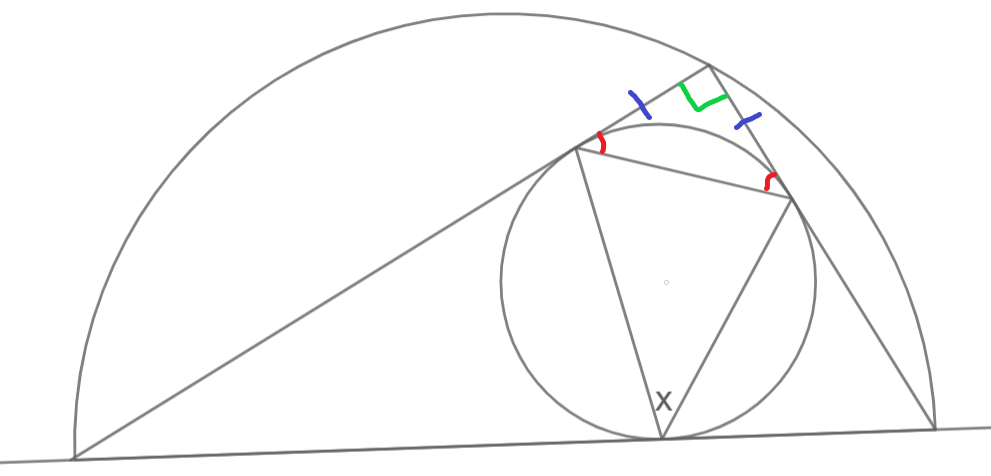
\includegraphics[scale=0.4]{angle_diagram_sol.png}
\end{center}
\textit{Note: The outer arc is a semicircle.}

{\itshape Because of the semicircle, we know that the green angle is $90^{\circ}$. We know that the blue lines are equal since they are tangents from a point. Thus, the red angles are equal as the triangle is isosceles. Using the sum of the angles in this triangle, we get the red angles as $45^{\circ}$ each. Finally, tan-chord gives $x=45^{\circ}$.}


\item % Tim
You are given a ${k\times k}$ chessboard. You are told that there is a square on the chessboard where, if you place a queen, you will not be able to place a knight anywhere else such that both of them don't attack each other. Assuming this to be true, what is the maximum possible value of $k$?

\begin{center}
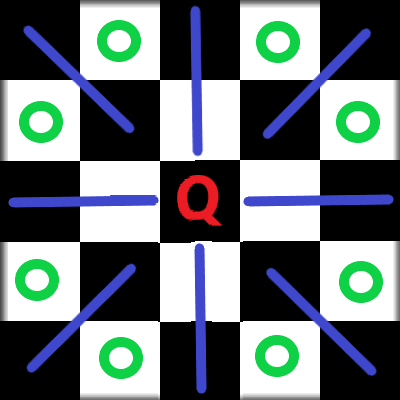
\includegraphics[scale=0.5]{chess.png}
\end{center}

{\itshape In the figure, we see that such a square exists for $k=5$. For $k=6$, no matter where we place a queen, we can guarantee that there will be a square exactly one square up or down from the queen and exactly three squares left or right. Placing a knight here will guarantee neither of them can attack each other. Thus, the maximum such $k$ is $k=5$.}


\item % Tim
Find all pairs of positive integers $(n,k)$ satisfying $$n^3=(7k+3)^2$$

{\itshape $n^3 = -1,0,1$(mod 7) while $(7k+3)^2 = 2$ (mod 7). Thus there are no such pairs.}


\item % Tim
There is a group of 6 people that are very suspicious of each other. It is very important to these people which of the rest of the group consider them to be friends. Now, because of the nature of this group, friendship is not a two way street! Person A may consider himself friends with Person B while Person B does not consider the same about Person A. A true friendship is a pair of people who both consider each other to be friends. If we are told that each of these 6 people considers exactly 3 others to be their friend, what is the maximum number of true friendships that can exist among these 6 people?

{\itshape Since each person considers 3 others to be their friends, we have $6\times 3 = 18$ considerations. This means that, since each true friendship contains two considerations, we can have at most 9 true friendships. To construct this, just call the people $A,B,C,D,E,F$ and connect every pair of true friends: }
\begin{center}
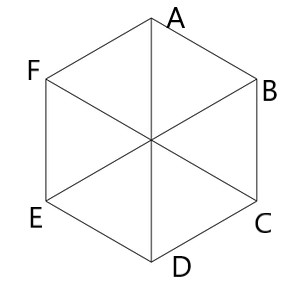
\includegraphics[scale=0.7]{graph.jpg}
\end{center}


\item % Tim
Considering the sequences $a_n$ and $b_n$:
\begin{itemize}
\item $a_1=2$ and $b_1=3$
\item $a_{n+1}$ is obtained by taking the sum of the squares of the digits of $a_{n}$
\item $b_{n+1}$ is obtained by taking the sum of the squares of the digits of $b_n$
\end{itemize}
Find the maximum value of $gcd(a_k,b_k)$ for any integer $k\geq 1$, and find all $k$ where this maximum value occurs.\\
\textit{Note: gcd is greatest common divisor, which is the same as highest common factor.}

{\itshape Expand the two sequences:\\
Sequence 1: $$2,4,16,37,58,89,145,42,20,4,16,37,58,89,145,42,...$$ Sequence 2: $$3,9,81,65,61,37,58,89,145,42,20,4,15,37,58,89,...$$ Noting that these patterns repeat with the same cycle length, we just need to check the first few $gcd$s and get $gcd(145,58)=29$. This occurs for $k=8a-1$ where $a\in \mathbb{Z}$ for $a\geq 1$.}


\item % British MO 2013/14 Round 1
In the acute-angled triangle $ABC$, the foot of the perpendicular from $B$ to $CA$ is $E$. Let $l$ be the tangent to the circumcircle of $\triangle ABC$ at $B$. The foot of the perpendicular from $C$ to $l$ is $F$. Prove that $EF$ is parallel to $AB$.


\item % Taariq
Let $x$ and $y$ be distinct real numbers such that $$x + 4 = (y - 2)^2 \quad\text{and}\quad y + 4 = (x - 2)^2$$
Find $x^2 + y^2$.


\item % Tim
\textbf{Bonus Question (from Advanced Test):}
A square-based pyramid has all of its edges the same length.
A cube is placed inside so that one of its faces lies on the base of the pyramid, and the opposite face has an edge along each side of the pyramid (think -- the natural way to put a cube in a pyramid).
Show that the sum of any of the cube's edge lengths with any of the cube's face diagonal lengths is the same as the edge length of the pyramid.

\begin{center}
\includegraphics[scale=0.5]{pyramid.png}
\end{center}
{\itshape Let the edge length of the pyramid be $s$ and the cube be $a$. Let $H$ be the foot of the perpendicular from $B$ to the base of the pyramid. Since H is the intersection of the base diagonals, we have $AH=HD$ and $A\hat{H}D=90^{\circ}$. Then Pythagoras gives $AH=\frac{s}{\sqrt{2}}$. A similar argument gives $GH=\frac{a}{\sqrt{2}}$. Note that $BH=\sqrt{AB^2-AH^2}=\frac{s}{\sqrt{2}}$. Now, we have $\triangle AGC \sim \triangle AHB$ since $GC\parallel HB$ in the plane $AGC$ ($CG$ is $\perp$ to the plane $AHD$). But this means $AG=GC$, since $AH=HB$. So $AG+GH=AH$ becomes $a+\frac{a}{\sqrt{2}}=\frac{s}{\sqrt{2}}$. So $\sqrt{2}a+a=s$. But the edge length of the cube is ${a}$, the face diagonal is $\sqrt{2}a$, and the edge length of the pyramid is $s$. Kapow.}

\end{enumerate}


\vfill
% ASCII art
\centering
\begin{BVerbatim}
>o)
(_>
\end{BVerbatim}

\end{document}